\documentclass[oneside, class=book, 12pt, crop=false]{standalone}

\usepackage{../dissertationstyle}

\bibliography{../personal}

\begin{document}

\ifstandalone
  \setcounter{chapter}{1}
  \chapter{Preparation}
\fi
\resetfigpath{preparation}


Structure:

Explain 

Talk about data collection (which pieces were used)

Talk about preparatory work done for understanding DSP techniques, as well as Ellis' beat-tracking system.

Choice of metrics: mention not using symbolic data makes it more difficult to get metrics that work has previously been done on

Requirements analysis:


remember:

reverb, echo, non-linear frequency response, fix by multiplying by inverse?


%%%%%%%%%%%%%%%%%%%%%%

This chapter gives and discuss the preparatory work done for this project. Before work began on the project, I had minimal knowledge in fields like digital signal processing (DSP) or music information retrieval (MIR).

\section{Digital Signal Processing Techniques}\label{section:dsp techniques}

First, we introduce some important DSP concepts and techniques: the Fourier transform, the discrete time Fourier transform, the discrete Fourier transform, and the mel scale.

In DSP, we can model an analog signal as a continuous function of time $x(t)$, and a digital signal as a discrete sequence $\{x_n\} = \ldots, x_{-2}, x_{-1}, x_0, x_1, x_2, \ldots$, essentially a list of numbers. With a sampling period $t_s$ we can sample an analog signal $x(t)$ to generate a digital signal $\{x_n\}$ as follows: $\{x_n\} = x(nt_s)$, or equivalently with sampling period $f_s$ we get $\{x_n\} = x(\frac{n}{f_s})$

\subsection{The Fourier Transform}\label{section:fourier transform}

An important operation in DSP is the Fourier transform, which allows us to convert a signal from the time-domain into the frequency-domain. The Fourier transform $X(f) = \mathcal{F}\{x(t)\}$ is defined  on a continuous signal $x(t)$ in Equation \ref{eq:ft}

\begin{equation}\label{eq:ft}
  X(f) = \mathcal{F}\{x(t)\}(f) = \int_{-\infty}^\infty x(t)e^{-j2\pi ft}\mathrm{d}t
\end{equation}

Here, the symbol $j$ refers to $\sqrt{-1}$. By rewriting $e^{-j2\pi ft}$ as $\cos(2\pi f t) - j\sin(2\pi f t)$ we get the definition in Equation \ref{eq:ft2}, which should make the purpose of this transform clearer:

\begin{equation}\label{eq:ft2}
  X(f) = \mathcal{F}\{x(t)\}(f) = \int_{-\infty}^\infty x(t)[\cos(2\pi ft) - j\sin(2\pi f t)] \mathrm{d}t
\end{equation}

Here, it is more obvious that we are taking the frequency content of $x(t)$. It should be noted that the Fourier transform generates complex values. However, if the signal $x(t)$ is both real and even, then its Fourier transform $X(f)$ will also be real and even. Subsequently, if $X(f)$ is real and even, then the values for negative $f$ contain the same information as the values for non-negative $f$, so we can purely consider real, non-negative frequencies, which makes interpreting the Fourier transform in a real-world sense easier.

As an example, we provide the Fourier transform of the box function in Figure \ref{fig:ft example}.

\begin{minipage}{\textwidth}
\begin{minipage}{.5\textwidth}
    \begin{tikzpicture}[
      declare function={
          func(\x)= (\x<=-1) * (0)   +
         and(\x>-1, \x<=1) * (1)     +
         (\x>1) * (0);
      }
    ]
    \begin{axis}[
      axis x line=middle, axis y line=middle,
      ymin=-1, ymax=2, ytick={-1,...,2}, ylabel=$x(t)$,
      xmin=-2, xmax=2, xtick={-2,...,2}, xlabel=$t$,
    ]
    % lol
    \addplot[blue, domain=-2:2, samples=100]{func(x)};
    \end{axis}
    \end{tikzpicture} 
\end{minipage}%
\begin{minipage}{.5\textwidth}
    \begin{tikzpicture}[
      declare function={
          func(\x) = sin(deg(\x))/(\x);
      }
    ]
    \begin{axis}[
      axis x line=middle, axis y line=middle,
      ymin=-1, ymax=2, ylabel=$X(f)$,
      xmin=-10, xmax=10, xlabel=$f$,
    ]
    % lol
    \addplot[blue, domain=-10:10, samples=100]{func(x)};
    \end{axis}
    \end{tikzpicture} 
\end{minipage}
\captionof{figure}{The rectangular function and its Fourier transform}\label{fig:ft example}
\centering
\end{minipage}


\subsection{The Discrete Time Fourier Transform and Discrete Fourier Transform}

For our work, we do not use continuous signals, we instead work with discrete sequences, and as such we need a variant of the Fourier transform to work with these discrete sequences. This is called the discrete time Fourier transform (DTFT), and the definition given in Equation \ref{eq:dtft} comes from considering our discrete sequence $\{x_n\}$ as being sampled from some continuous signal at sampling frequency $f_s$:

\begin{equation}\label{eq:dtft}
  \hat{X}(f) = \mathcal{F}\{\{x_n\}\}(f) = \sum_{-\infty}^\infty x_n \cdot e^{-2\pi j \frac{f}{f_s}n}
\end{equation}

In practice, we make one further restriction on our input sequences: they are finite. Fortunately, a useful property of the Fourier transform (that also holds for the DTFT) is that if the input is periodic, then the resulting spectrum will be discrete. So, we can take our finite input sequence, and turn it into an infinite, periodic, discrete sequence, and then take the DTFT to get a discrete frequency spectrum, which gives us the discrete Fourier transform (DFT).

This does not require much work to calculate, and for a finite sequence $x_0, \ldots, x_{N-1}$, we simply replace the bounds on our sum in Equation \ref{eq:dtft} with 0 and $N-1$, to get the definition of the DFT in Equation \ref{eq:dft}:

\begin{equation}\label{eq:dft}
  X_k = \sum_{n=0}^{N-1} x_n e^{-2\pi j \frac{k}{N}n}
\end{equation}

\subsection{Convolution}

%TODO


\subsection{The Mel Scale}

The mel scale is a scale of frequencies that intends to map distance between frequencies to differenecs in perceptual pitch. This is useful for this project, since the quantity we actually care about is pitch, and not Hertz frequency.

There are many different definitions for the mel scale, since perceptual pitch is a relatively subjective meausre, but we use the definition in Equation \ref{eq:mel}, where $f$ is a frequency in Hertz and $m$ is the corresponding frequency in the mel scale:

\begin{equation}\label{eq:mel}
  m = 2595\log_{10}\left(1 + \frac{f}{700}\right)
\end{equation}

\section{Beat Tracking}

Beat tracking is the technique of taking some audio signal of music, and attempting to find the location of beats, or the pulse, of the music. This is not the same as rhythm, since rhythm is more concerned with the location of individual notes, whereas beats are a steady pulse perceived by humans throughout a whole piece of music. The technique we use for beat tracking comes from a paper by Ellis \cite{ellis07} and makes use of dynamic programming techniques.

To perform beat tracking, we assume the existence of some onset function and a global tempo estimate, Ellis' constructions of which we explore further in Sections \ref{subsec:onset detection} and \ref{subsec:tempo inference} respectively. An onset function tracks where perceptual note onsets are in an audio signal as seen in Figure \ref{fig:onsetfunction}, and a tempo estimate is simply an estimate of how fast the piece is being played overall, in beats per minute (BPM).

QUESTION: is it worth explaining this algorithm in large detail? or just direct the reader to Ellis' paper, don't want to plagiarise.

The dynamic programming algorithm for beat tracking works by assuming we have some already optimal set of previous beat times, and then searching for the next beat time by trying to find a time with a high onset function value, as well as being coherent with the tempo estimate.



\begin{minipage}{\textwidth}
  \centering
  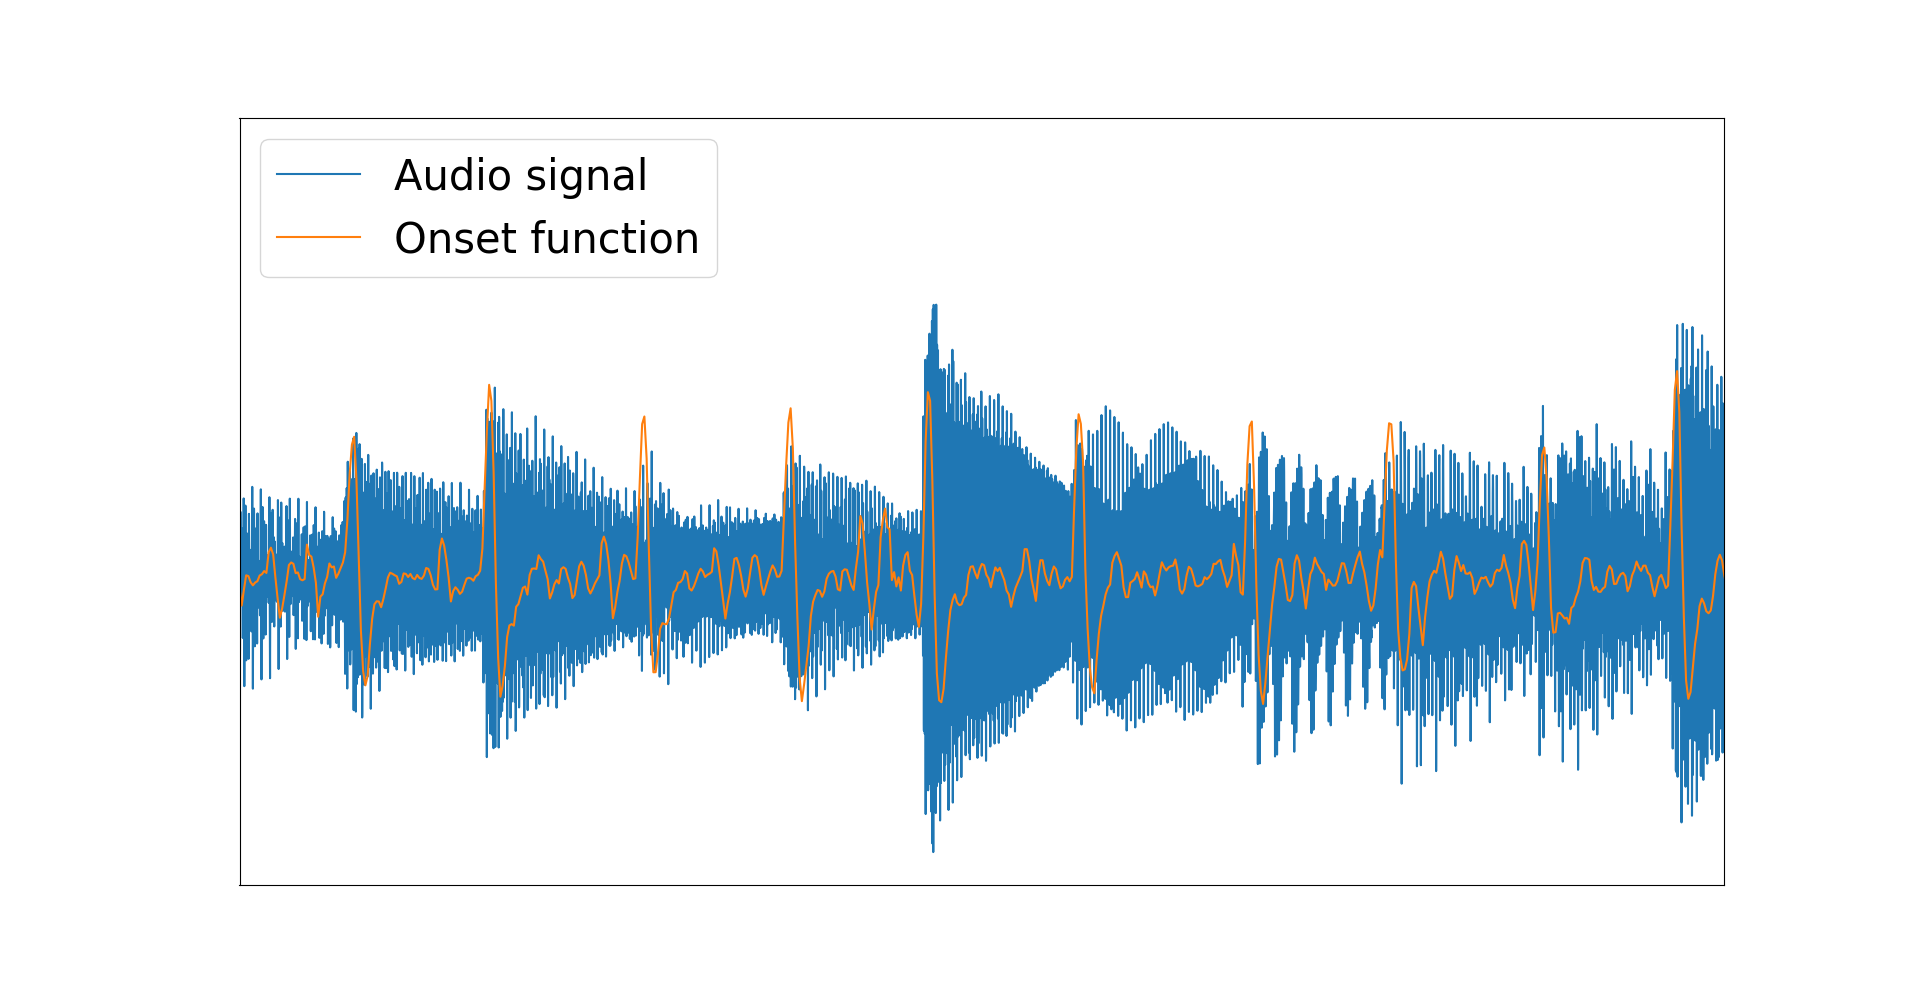
\includegraphics[scale=0.3]{onsetfunction}
  \captionof{figure}{Example onset function against audio signal}\label{fig:onsetfunction}
\end{minipage}

\subsection{Onset Detection}\label{subsec:onset detection}

 There is a wide literature on onset detection \cite{bello05}, but due to the nature of the relevant audio recordings (solo piano performances) which are relatively simple and have strong percussive elements, opting for the simple technique used by Ellis seemed sensible.

 The idea behind Ellis' onset function is to report a high value when there are large jumps in energy in multiple frequency bands, which indicates a note has been played.

 The technique works as follows:

 \begin{itemize}

   \item
     First, resample the signal to 8kHz (this means we will not be able to detect frequencies above 4kHz, which is good because the highest frequency note a piano can generate is $\sim$4kHz)

   \item
     Take windows of the sound, we use a 32ms wide window and advance by 4ms.

   \item
     For each window, compute its DFT.

   \item
     Convert the frequencies in the DFT to use the mel scale instead of Hertz, to more accurately represent pitch bands.

   \item
     Convert the amplitudes in the DFT to use dB for normalisation.

   \item
     Across all windows, compute the first-order difference for each pitch band, setting negative values to zero (so they do not interfere with the next step)

   \item
     For each pair of windows, sum all of the first-order differences together, such that we get a signal.

   \item
     To make this signal have zero-mean (like a regular signal would), we pass the signal through a high-pass filter with a cutoff at 0.4Hz

   \item
     To smooth the signal, we convolve it with a small Gaussian distribution.

   \item
     Finally, we normalise the signal by dividing by the standard deviation.

 \end{itemize}

 The output of this is our onset function $O(t)$


 \subsection{Tempo Inference}\label{subsec:tempo inference}

 The tempo inference algorithm is relatively simple, and uses our onset function.

 The idea is to try many potential values $\tau$ that represent the expected distance between each beat (the corresponding tempo would be $\frac{60}{tau}$). Then, we compute $O(t-\tau)$ and take the inner product with $O(t)$. If $\tau$ is a good guess, then this inner product will be high, since many peaks in the onset function will line up.

 It is important to note that we cannot simply choose the $\tau$ that gives us the highest inner product, since this could find many valid tempos. For instance, if 80 BPM is our actual tempo, then 40 BPM, 20 BPM, etc. will be equally as good estimates.

 To solve this issue, we apply a weighting function to each $\tau$ that corresponds to the likelihood that a human would choose this tempo out of all valid tempos. In particular, we center around 120 BPM and drop off either side, as shown in Figure \ref{fig:tempo weighting function}.

 The exact formula is given as follows in Equation \ref{eq:tempo weighting function}

 \begin{equation}\label{eq:tempo weighting function}
   W(\tau) = \exp\left(-\frac{1}{2}\left(\frac{\log_2 \frac{\tau}{\tau_0}}{\sigma_\tau}\right)^2\right)
 \end{equation}

 In this equation, $\tau_0$ is our tempo bias, so 0.5 (corresponding to 120 BPM). $\sigma_\tau$ is how fast our weighting function drops off, and is set at 1.4 corresponding to empirical measurements done by Ellis.




\begin{minipage}{\textwidth}
  \centering
    \begin{tikzpicture}
    \begin{axis}[
      axis x line=middle, axis y line=middle,
      ymin=0, ymax=1.5, ytick={-1,...,1}, ylabel=$W(\tau)$,
      xmin=0, xmax=3, xtick={0,...,3}, xlabel=$\tau$,
    ]
    % lol
    \addplot[blue, domain=0:3, samples=100]{exp(-0.5 * ((log2(x / 0.5)) / 1.4)^2)};
    \addplot [mark=none,dashed, black] coordinates {(0.5, 0) (0.5, 1)};
    \node[label={90:{(0.5, 1)}}, circle, fill,inner sep=2pt] at (axis cs: 0.5,1) {};
    \end{axis}
    \end{tikzpicture} 

    \captionof{figure}{$W(\tau)$}\label{fig:tempo weighting function}
\end{minipage}%


\ifstandalone
  \printbibliography
\fi
    
\end{document}
